\documentclass{standalone}
% Load any packages needed for this document
\begin{document}

\section{Chapter 1: Introduction into Virtual Reality}

\setcounter{subsection}{1}	% 1.1 omitted

%----------------------------------------------------------------------------------------
\subsection{The development of the computer}

\begin{itemize}
	\item \textbf{the constant increase of computational power available in modern computer} $\rightarrow$ today's abundance of virtual reality. 
\end{itemize}

\subsubsection*{Numbers}
\begin{itemize}
	\item 6000 years ago: the earliest use of numbers. 
		\begin{itemize}
			\item 3300 B.C. Egypt: battle report in hieroglyphs.
		\end{itemize} 
	\item number system 
		\begin{itemize}
			\item The first number systems exist in hieroglyphs \\ e.g. $1=\textit{line}$, $10=\textit{horseshoe}$ ...
			\item Roman: 

				\begin{table}[h]
				\centering
				\begin{tabular}{| c | c | }
				\hline
				I $= 1$		& V $= 5$ 	\\
				\hline 
				X $= 10$	& L $= 50$ 	\\
				\hline							
				C $= 100$	& D $= 500$ \\
				\hline					
				M $= 1000$ 	& 			\\		
				\hline					
				\end{tabular}
				\end{table}
				
				\begin{center}
				$2388 =$ MMCCCLXXXVIII
				\end{center}
			
			\item \textbf{Addition-system} (Roman, Greeks, Syrians, Slavic tribes ...): large numbers are made by adding up the symbols 
			\item \textbf{Indo-Arabian}: the system used until today (1, 2, 3, 4, 5, 6, 7, 8, 9, 0)
				\begin{itemize}
					\item more complicated calculation can be performed very easily.
					\item very forgery-proof
					\item 6th century: Indian to Mesopotamia (Severus Sebakt)
					\item 10th century: came to Europe (Leonardo Fibonacci)
					\item 16th century: printing numbers were introduced (Adam Ries and Albrecht Dürer) 
				\end{itemize}				
		\end{itemize}
\end{itemize}

\subsubsection*{Calculation}

\begin{itemize}
	\item First means to calculate
		\begin{itemize}
			\item calculating with the fingers - Rome: 40 finger positions, displays up to 200000 (Note: digitus(finger in Latin) $\rightarrow$ digit (eng.))
			\item tally stick (Europe), knots (native Americans)
		\end{itemize}
	\item The first scientific calculation: \textbf{abacus} 
	\item \textbf{Written calculation became popular (since 15c)}
		\begin{itemize}
			\item \textbf{easy and fast}: eased calculations and reduced the required time.
			\item \textbf{accurate}: lowered the failure rate.
			\item Adam Ries: make math accessible to everybody.
		\end{itemize} 
\end{itemize}

\subsubsection*{Calculation machine (17c $\sim$)}

\begin{itemize}
	\item to make calculation more easy, fast and accurate
	\item the first calculation machine (W. Schickardt, 17c) \textbf{Figure 1.16, page 1-12}
		\begin{itemize}
			\item add numbers up to 6 digits
			\item multiplication were possible. 
			\item toothed gears and slide rules. 
		\end{itemize}
	\item B. Pascal(1623 - 1662) \textbf{Figure 1.17, page 1-12}
		\begin{itemize}
			\item made money with calculation machine (the first one) 
			\item add and subtract numbers with 8 digits. 
			\item more than 50 pieces were produced. 
		\end{itemize}
	\item G. W. Leibniz (1646 - 1716) \textbf{Figure 1.18, page 1-12}
		\begin{itemize}
			\item introduced the machine suitable for all four basic calculation. 
		\end{itemize} 
	\item The calculating machines of 18c: more reliable, but became a piece of jewelry than a device for daily use \textbf{Figure 1.19, page 1-13}
	\item C. X. Thomas (1785 - 1870) \textbf{Figure 1.20, page 1-13}
		\begin{itemize}
			\item precise, efficient and ergonomic.
			\item ``arithmometer": multiplied two numbers with 8 digits in 18 sec.
			\item more improved later 	
		\end{itemize}
	\item \textbf{Programmable calculation machines} (C. Babbage, 1792 - 1871)
		\begin{itemize}
			\item punched cards for \textbf{programming.} 
			\item could run the program autonomously.
			\item used steam machine and weights, but failed to realize his idea. 
			\item \textbf{separated counting mechanism, calculation mechanism and storage} (origin of 20c computer architecture)
		\end{itemize}
	\item \textbf{Calculation machine with electrical devices} (H. Hollerith, 1860 - 1929)
		\begin{itemize}
			\item \textbf{Figure 1.22, page 1-15}
			\item control mechanism activated by electrical devices (relays, motors ... ) with punched cards: hole $\rightarrow$ closed (1) / no hole $\rightarrow$ opened (0)
			\item American Census in 1890: shorten the time for analysis 7 yrs $\rightarrow$ 1 yrs
			\item founded IBM
		\end{itemize}
\end{itemize}

\subsubsection*{Computer era (20c $\sim$)}

\begin{itemize}
	\item Theoretical background of the first programmable electrical calculation machine (The first computer): \textbf{L. Couffignal and A. M. Turing}
	\item The first computer: \textbf{ZUSE Z3} by K. Zuse (1941)
		\begin{itemize}
			\item Z1 (didn't work) $\rightarrow$ Z2 (simple tests) $\rightarrow$ Z3 
			\item could handle 64 numbers with 22 digits. 
			\item 2600 relays and 8 line punched tape ($\rightarrow$ tube/transistor was used later)
			\item Z4 (1950s) worked at ETH 
		\end{itemize}	
	\item \textbf{The first encryptor \& decryptor}: Enigma vs Colossus (1941)
		\begin{itemize}
			\item Colossus: \textbf{the first electronic computer}
				\begin{itemize}
					\item MARK 1 (1943) in US
					\item MARK 2 (1944) in US
				\end{itemize}
		\end{itemize} 
	\item \textbf{ENIAC (1946)} \textbf{Figure 1.25, page 1-16}
		\begin{itemize}
			\item J. P. Eckert, J. Mauchley and H. H. Goldstine
			\item \textbf{von Neumann architecture}
			\item first electronic computer? (vs Colossus. actually not)
			\item 18000 tubes, 1500 relays, 1000 capacitors and 6000 switch.
			\item very fast... 0.0002 sec for addition, 0.0028 sec for multiplication 
		\end{itemize}
	\item \textbf{Transistor} invented (1948) \textbf{Figure 1.26, page 1-17}
		\begin{itemize}
			\item \textbf{smaller, faster, less heat, longer life cycle, manufactured automatically}
			\item \textbf{switch: relays $\rightarrow$ tubes $\rightarrow$ transistor} (electronics)
			\item TRADIC (1955): the first computer used transistors
		\end{itemize}   
	\item \textbf{single chip computer(CPU)} (Integrated Circuits) 
		\begin{itemize}
			\item 4-bit processor INTEL and Texas Instrument in 1970
			\item 8-bit (1972), 16-bit (1978) ... now 32 bit / 64 bit
		\end{itemize}
	\item \textbf{Personal Computer (PC)}
		\begin{itemize}
			\item because of IC, the size of computers could be drastically reduced
			\item Kenbak1 (1971): the first single chip computer
			\item ALTAIR 880 (1974): mass market
				\begin{itemize}
					\item \textbf{Basic}: a new programming language developed for ALTAIR
				\end{itemize}
			\item (1980s) Apple II \& Commodore PET: the first commercial success
			\item Lisa and Macintosh : GUI
			\item IBM PC became very popular
		\end{itemize}
	\item SGI were used for high-performance computer graphics: Virtual Reality...
\end{itemize}

\subsubsection*{Moore's law and the development of computer}

\begin{itemize}
	\item \textbf{Moore's law} (1965): \textbf{the amount of transistors} in a computer is doubled all 18 months. \textbf{Figure 1.34, page 1-22}
	\item but also the required space for the transistors becomes smaller and smaller. i.e. \textbf{the available memory per chip} is increases: x4 every 3 yrs
	\item \textbf{chip size} also increases: x2 every 10 yrs 
	\item \textbf{CPU speed} increases: x2 every year
\end{itemize}

\begin{figure}[H]
	\centering
	\begin{subfigure}[b]{0.45\textwidth}
		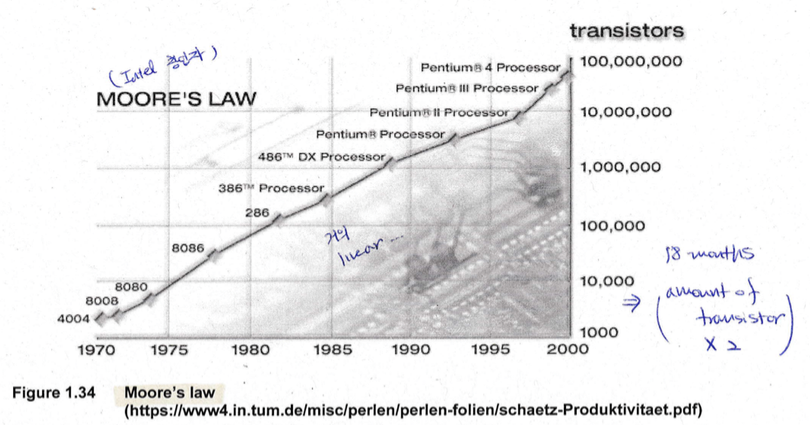
\includegraphics[width=\linewidth]{1_34}
	\end{subfigure}
	\begin{subfigure}[b]{0.45\textwidth}
		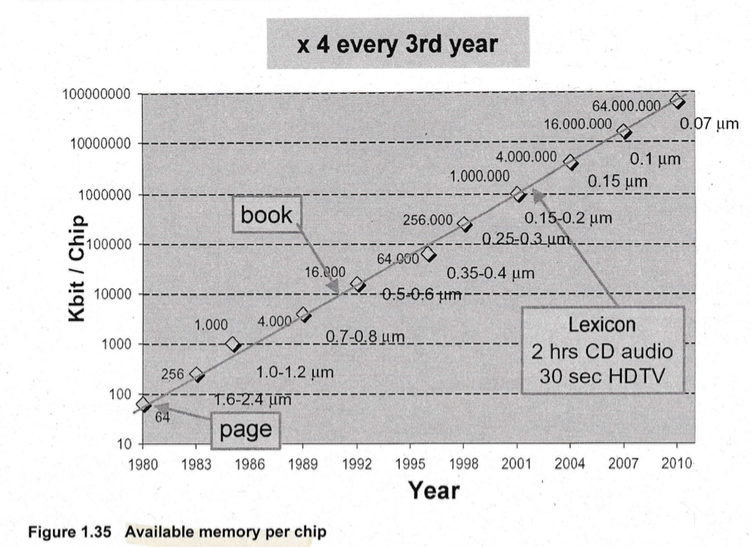
\includegraphics[width=\linewidth]{1_35}
	\end{subfigure}
	\begin{subfigure}[b]{0.45\textwidth}
		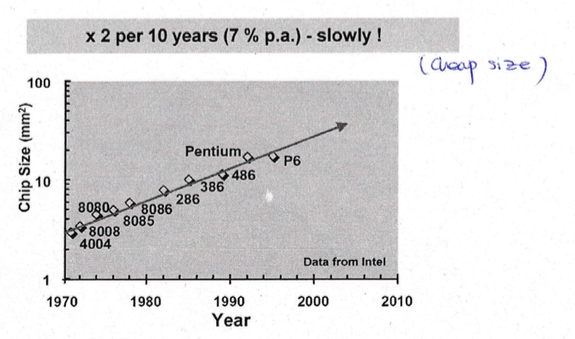
\includegraphics[width=\linewidth]{1_36}
	\end{subfigure}
	\begin{subfigure}[b]{0.45\textwidth}
		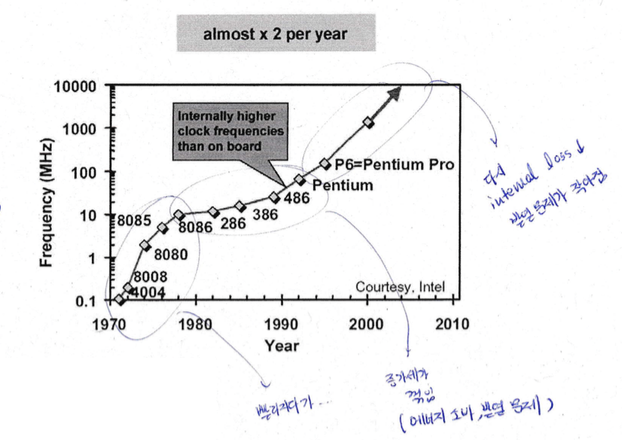
\includegraphics[width=\linewidth]{1_37}
	\end{subfigure}
\end{figure}

\subsection{Definitions}

\begin{itemize}
	\item Reality (exist): real object $\gg$ virtual object
	\item Mixed Reality 
		\begin{itemize}
			\item Extended Reality (Augmented Reality): real obj $>$ virtual obj
			\item Extended Virtuality (Augmented Virtuality): real obj $\leq$ virtual obj
		\end{itemize}
	\item Virtual Reality (non exist): real obj $<$ virtual obj
	\item \textbf{Note: Figure 1.39, page 1-25}
\end{itemize}

\begin{figure}[H]
	\centering
	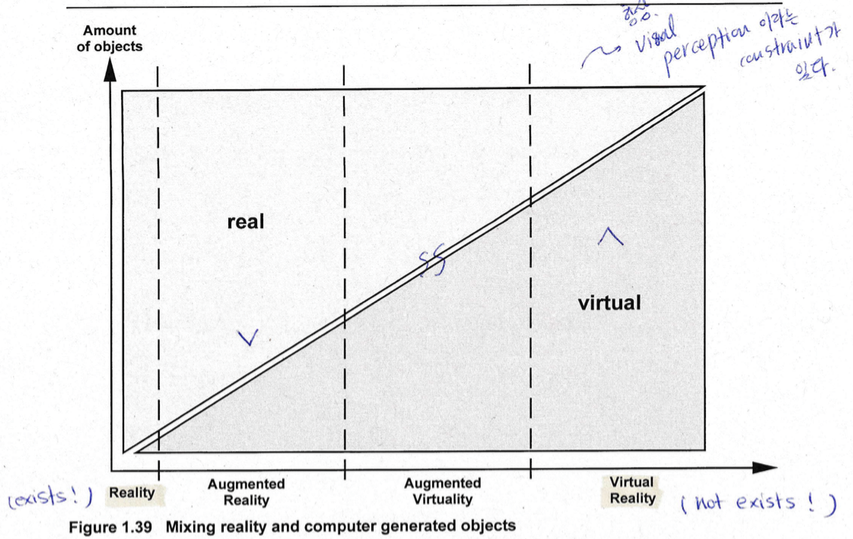
\includegraphics[width=\linewidth]{1_39}
\end{figure}

\subsubsection{Extended Reality (augmented reality)}

\begin{itemize}
	\item \textbf{real object $>$ virtual object}
	\item the computer generated objects are characterized by the fact but usually differ from reality in scale, shape or color.
	\item e.g. AR on copy machine: indicate parts to be fixed  
\end{itemize}

\subsubsection{Extended Virtuality (autmented virtuality)}

\begin{itemize}
	\item \textbf{real object $<$ virtual object}
	\item comparing to AR, virtual objects are much more detailed and fit much better to reality.
	\item e.g. Reconstruction of ruins \textbf{Figure 1.40}
\end{itemize}

\subsubsection{Virtual Reality}

\subsubsection*{Definition}

\begin{itemize}
	\item Former Definition: a possible or considered reality, \underline{which is not available yet.}
	\item Complete Definition: \textbf{``Virtual Reality is a computer generated, interactive and three-dimensional environment, in which the user is completely immersed"}
		\begin{enumerate}
			\item a fictive and non-real world (e.g. TV, movie, dream are fictive and non-real world)
			\item ``cybernetic room" or ``cyberspace": controllable and manageable room, in which information is processed. (e.g. chess, board games)
			\item generated by computer, using specialized program: imaginary reality can only be reached by processing numerous infos. 
		\end{enumerate}
\end{itemize}

\subsubsection*{The VR reference model}

\begin{itemize}
	\item \textbf{Figure 1.41, page 1-27}
	\item Three component (three axis)
		\begin{itemize} 
			\item interaction (none $\rightarrow$ interactive $\rightarrow$ immersive)
			\item semantics of data (none $\rightarrow$ static $\rightarrow$ dynamic)
			\item presentation (single event $\rightarrow$ sequence of events $\rightarrow$ real time)
		\end{itemize}
	\item optimal VR application $=$ \underline{immersive interaction} $+$ \underline{dynamic semantics} $+$ \underline{real time presentation} 
	\item Note, but not each VR application requires the maximum amount of all three criteria.
\end{itemize}

\begin{figure}[h]
	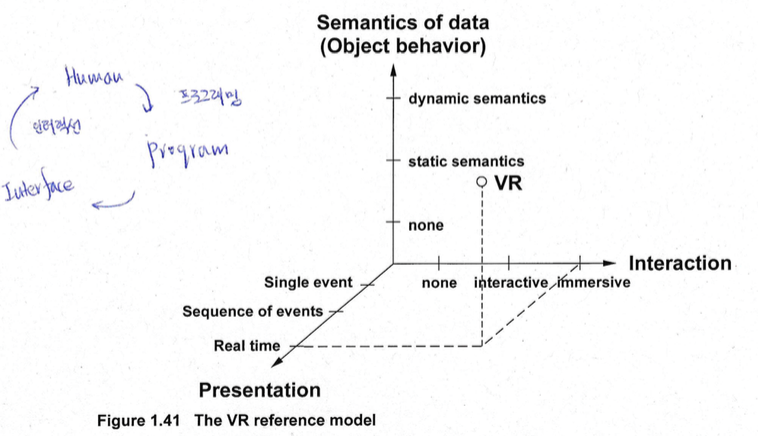
\includegraphics[width=\linewidth]{1_41}
\end{figure}

\subsubsection*{I$^3$ - Immersion - Interaction - Imagination}

\begin{itemize}
	\item technology provided by VR ...
		\begin{itemize}
			\item is used to immerse into the virtual env. (immersion)
			\item is used to interact with its objects. (interaction)
			\\ $\rightarrow$ VR addresses all perception channels of the user and thus he is convinced of the reality of VR env. (imagination)
		\end{itemize}
	\item i.e. Two prerequisites for VR: immersion \& interaction (\textbf{immersion \& interaction} $\rightarrow$ imagination)
	\item \textbf{latency time should be smaller than 0.1 sec!}
\end{itemize}

\begin{figure}[H]
	\centering
	\begin{subfigure}[b]{0.45\textwidth}	
		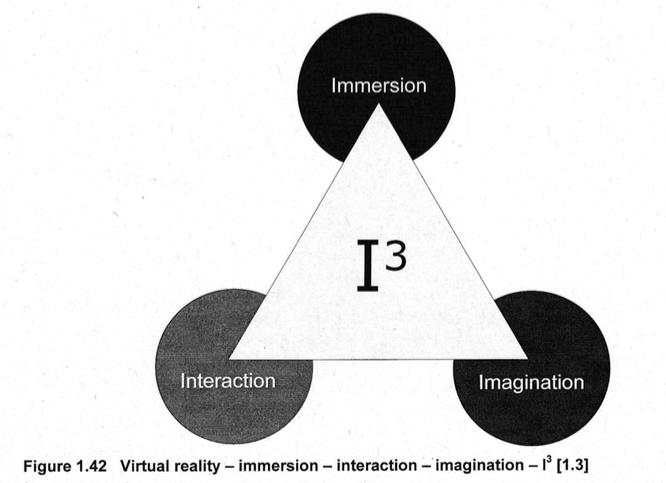
\includegraphics[width=\linewidth]{1_42}
	\end{subfigure}
	\begin{subfigure}[b]{0.45\textwidth}	
		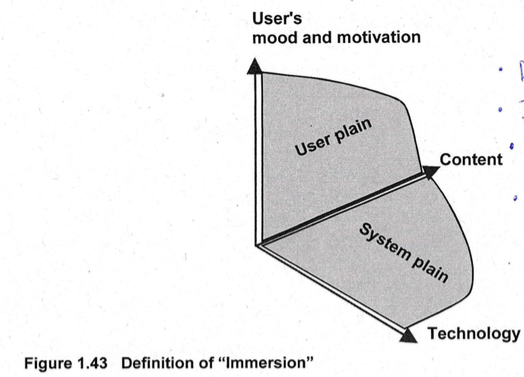
\includegraphics[width=\linewidth]{1_43}
	\end{subfigure}
\end{figure}

\subsubsection*{Interaction}

\begin{itemize}
	\item \textbf{interplay of information, action and reaction.}
	\item describes the effect of computer generated models onto the \textbf{human perception channels.} 
	\item continuous: continuous interaction with the virtual environment \textbf{(low delay)}
	\item reaction: every movement of the user causes a reaction in VR (note: difference with movies)
	\item generation / modification of geometry displayed, visual, acoustic, haptic, olfactory, and physical properties (e.g. collision, material prop., torque, DOF ...)of virtual object (copy or supplement real object)
	\item interactivity: ability of the system to allow a user's interaction, while the application is running. Special hardwares are needed.
	\item interaction facility 
		\begin{itemize}
			\item Passive: the user sees, hears and feel. (e.g. "Back to the Future" ride of Universal Studios)
			\item Exploratory: the user can explore the virtual env. 
			\item Interactive: the user explores the env, and interacts with the virtual objects also modify the env.
		\end{itemize}
\end{itemize}

\subsubsection*{Immersion}

\begin{itemize}
	\item Goal: to create the \textbf{``Sense of Presence" (SOP)} i.e. subjective impression of the user to be integrated in a fictive environment, which is not physically present.
	\item SOP focusing on...
		\begin{itemize}
			\item Natural interaction
			\item Interface to the computer is in the background
			\item Higher information density is possible
			\item More efficient access to complex data
		\end{itemize}
	\item User plain vs. System plain: interaction of both plains is the main purpose of supporting tech. Immersion is to map both plains onto each other.
\end{itemize}

\subsubsection*{Virtual Environment}

\begin{itemize}
	\item for interactivity, powerful computers are needed.
	\item sub-categories of virtual env.
		\begin{itemize}
			\item Reality driven virtual env.: generated model could also exist in reality
			\item Scaled virtual env.: computer generated which exists in reality, but can only be understood and explained by the user who applies the virtual model.
			\item Distant virtual env.: computer generated which represent a model of the real would cannot be explored out of distance or security reasons.
			\item Imaginative virtual env.: computer generated only come from the user's imagination.
			\item Informative virtual env.: visualize abstract data.
		\end{itemize}
	\item another sub-categories of virtual env.
		\begin{itemize}
			\item desktop virtual env.
			\item immersive virtual env.
			\item augmented virtual env.
			\item telepresence virtual env.
		\end{itemize}
\end{itemize}

\begin{figure}[H]
	\centering
	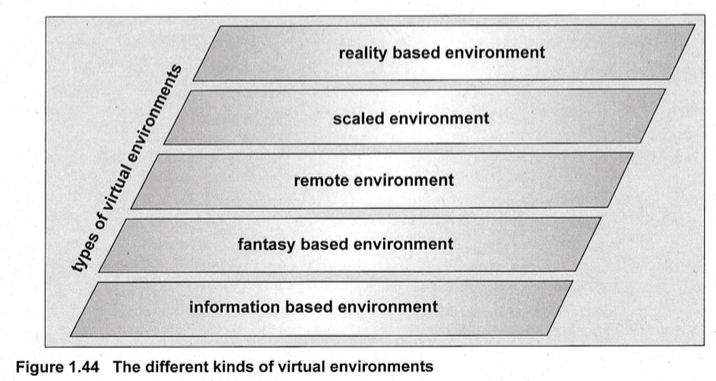
\includegraphics[width=0.6\linewidth]{1_44}
\end{figure}

\subsubsection*{Summary}

Virtual (VR) is a computer fictive world, which is characterized by the fact, that it can address \textbf{the perception channels} of the human user via interfaces. The user registers these sensations and answers by certain \textbf{reactions}. These reactions are registered by \textbf{the virtual environment} and cause corresponding reactions of the system. In order to complete the illusion of a new virtual reality, \textbf{only sensations from VR and not from reality can reach the user.} Thus, the user feels \textbf{completely immersed} in the virtual environment, which temporarily replaces reality. VR has to respond \textbf{fast and correctly} (corresponding to the defined rules) to the actions of the user.

\subsubsection{The Benefit of VR for industry}

\begin{figure}[H]
	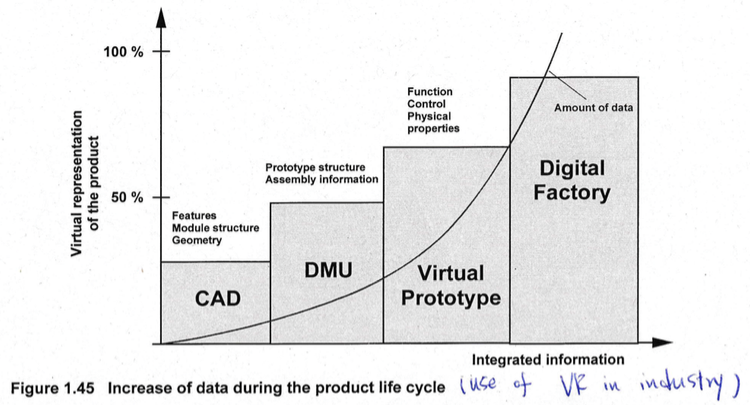
\includegraphics[width=\linewidth]{1_45}
\end{figure}

\begin{itemize}
	\item complexity of today's product $\rightarrow$ huge amount of data.
	\item product life cycle vs. data
		\begin{itemize}
			\item CAD: module geometry
			\item DMU(Digital Mock-up): assembly verification, collision detection and tolerance analysis
			\item Virtual prototype: physical properties (function simulation and software simulation)
			\item Digital factory: design and manufacturing process are considered
		\end{itemize}
	\item prototyping process up to now (physical mock-up)
		\begin{itemize}
			\item Digital proto $\rightarrow$ geometrical proto $\rightarrow$ functional proto $\rightarrow$ technical proto
		\end{itemize}
	\item now, VR is used for prototyping by DMU. (alternative of physical mock-up)
		\begin{itemize}
			\item \textbf{reach same quality of product in less time.} (Figure 1.47)
			\item \textbf{design modification iteration is much smaller and faster}: time \& cost-saving \\
				$\rightarrow$ much closer to ideal development process (Figure 1.48 and 1.49)
			\item all digital data gathered can be used later for other purposes (e.g. for the sales process)
			\item visualization of data: creative teamwork (idea generation)
		\end{itemize}
\end{itemize}

\begin{figure}[H]
	\centering
	\begin{subfigure}[b]{0.3\textwidth}	
		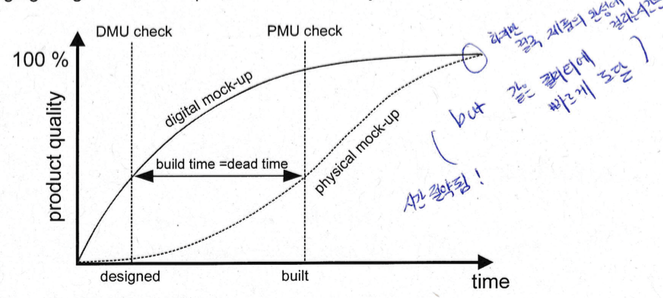
\includegraphics[width=\linewidth]{1_47}
	\end{subfigure}
	\begin{subfigure}[b]{0.3\textwidth}	
		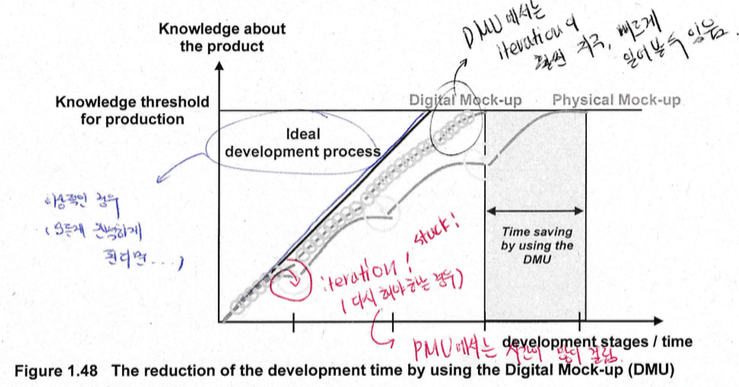
\includegraphics[width=\linewidth]{1_48}
	\end{subfigure}
	\begin{subfigure}[b]{0.3\textwidth}	
		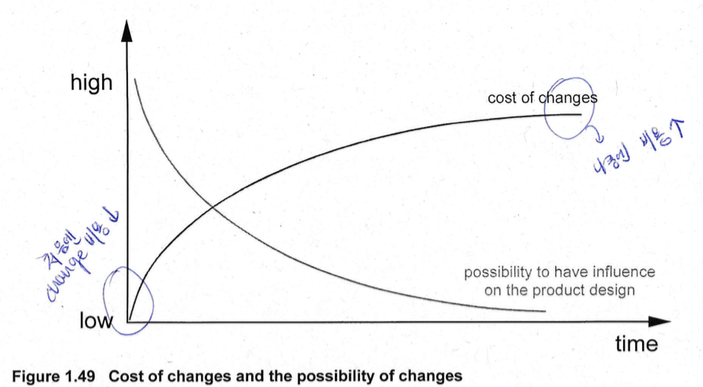
\includegraphics[width=\linewidth]{1_49}
	\end{subfigure}
\end{figure}

\subsubsection*{VR in product development process}

\begin{itemize}
	\item FMEA (Failure Mode and Effectiveness Analysis): visualization of geometry $\rightarrow$ detect possible failures, show the required details to all persons simultaneously.
	\item Access control: check accessibility to important point. (e.g. screw connections, connectors...: Figure 1.51)
	\item Kinematic verification: collision check w/o building (physical) proto.
	\item Design review: general design review. (geometrical proto)
	\item Crash simulation: automotive sector. Deformation process can be visualized.  
\end{itemize}

\subsubsection*{VR in Later production phases}

\begin{itemize}
	\item User training: for complex products, person can handle the product have to be taught in parallel. (e.g. escape from the plant in emergency)
	\item Product presentation: important part of the sales process. (e.g. Motor show)
	\item Assembly/service instruction: VR offers techniques and algorithms, which can drastically reduce the amount of data for complex geometries. (less powerful computer for visualization can be used.)
\end{itemize}

\subsubsection*{Digital product and services for user}

\begin{itemize}
	\item the structures of the digital product are optimized for the computer, not for the access by the user directly. 
	\item improvement of the interaction between the user and the digital product is a main requirement
	\item The user uses special \textbf{services} that allow him the access to the processes based on the digital product:
		\begin{itemize}
			\item visualize: content of the digital product or parts of it are visualized to the user. (graphical / text-based)
			\item simulate: unknown behavior will be simulated
			\item archive: all data about the product allows having instantaneous access to them
			\item document: documentation of a product or the processes (graphical / text-based)
			\item transfer: content of the digital product or excerpts of it are transferred over a network in a digital form
			\item present: excerpts of the digital product were extracted, processed and displayed. (optical aspects are in the focus of interest)
			\item integrate: excerpts of the digital product are integrated into the database. 
		\end{itemize}
\end{itemize}

\begin{figure}[H]
	\centering
	\begin{subfigure}[b]{0.45\textwidth}	
		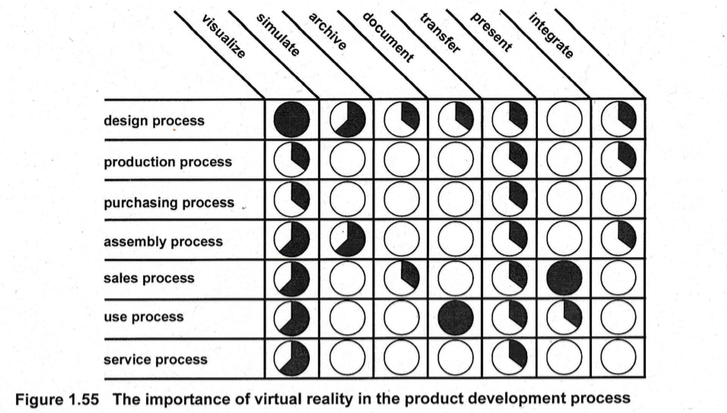
\includegraphics[width=\linewidth]{1_55}
	\end{subfigure}
	\begin{subfigure}[b]{0.45\textwidth}	
		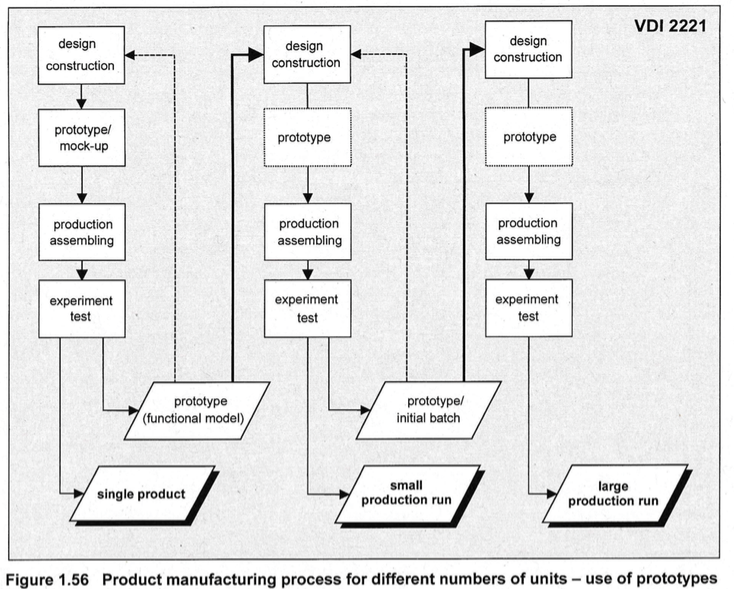
\includegraphics[width=\linewidth]{1_56}
	\end{subfigure}
\end{figure}


\subsubsection*{Real Prototypes and Mock-ups}

\begin{itemize}
	\item It is usual to pass the process several times and to create functional prototypes and initial batches.
	\item Benefit of using digital mock-ups (e.g. CAD, CAE)
		\begin{itemize}
			\item Communication: team works (e.g. marketing team $\leftrightarrow$ designer $\leftrightarrow$ process engineer)
			\item Documentation of the state-of-the-art: review the state-of-the-art of the product under development. (know-how reached so far and reduces uncertainties)
			\item Integration platform: integration of sub-systems. 
			\item Documentation of development steps (milestones): this can ensure the overall development goal can be achieved within a realistic time. 
		\end{itemize}
	\item New visualization technologies is to replace the physical proto. 
	\item VR allows the generation of synthetical environments in the computer for a realistic simulation of a design or construction.
	\item Digital mock-ups is in the dramatic reduction of development time, the higher product quality, and the reduction of cost for changes.
\end{itemize}

\begin{itemize}
	\item Note: classification of prototypes
		\begin{itemize}
			\item design proto: verification of the conceptual design concerning optical, esthetical, ergonomic requirements (not mechanical properties)
			\item geometrical proto: verification of dimensional, tolerances, and fits. (not material)
			\item functional proto: verification of mechanical, electrical, acoustical properties.
			\item technical proto: all functional. 
		\end{itemize}
\end{itemize}



\subsubsection*{Usage of VR and AR in the product development process}

\begin{itemize}
	\item VR - mainly at the beginning of the product's life cycle
	\item AR - increasing importance in the later stages 
	\item (the amount of VR decreasing) = (the amount of AR increasing)
	\item Note: at the present time, VR is a slight dominance. It's difficult to synchronize the real and the virtual object in time and position. (AR is much challenging)
\end{itemize}

\begin{figure}[H]
	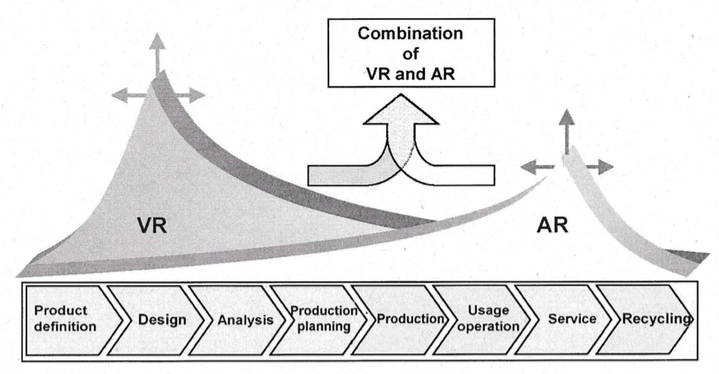
\includegraphics[width=\linewidth]{1_59}
\end{figure}

\end{document}